\begin{abwframe}
  % Faithful reconstruction of original PowerPoint slide 22 using its three
  % separately extracted visual objects, never a screenshot of the old slide.
  \node[anchor=north,text width=380bp,align=center,inner sep=0pt] at (255,-83)
    {{\TimesNR\fontsize{44}{50}\selectfont\bfseries\color{ABWRed}Big Data}};
  \node[anchor=north,text width=450bp,align=center,inner sep=0pt] at (700,-83)
    {{\TimesNR\fontsize{44}{50}\selectfont\bfseries\color{ABWRed}Big Calculations}};

  \node[anchor=north,inner sep=0pt] at (360,-186)
    {\href{https://ourworldindata.org/grapher/historical-cost-of-computer-memory-and-storage}{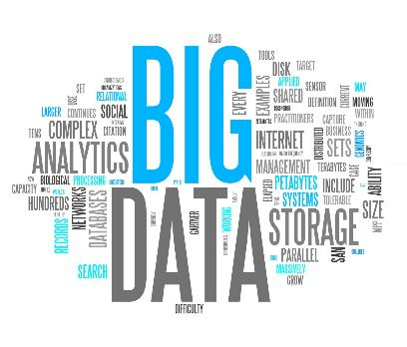
\includegraphics[width=290bp,height=290bp,keepaspectratio]{assets/visuals/lecture-1/slide-22-big-data-big-calculations-visual-03.png}}};
  \node[anchor=north,inner sep=0pt] at (713,-150)
    {\href{https://mobook.github.io/MO-book/notebooks/04/08-traveling-salesman-problem.html}{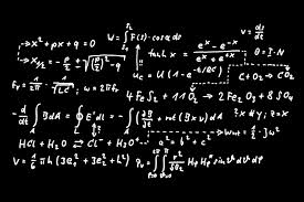
\includegraphics[width=380bp,height=170bp,keepaspectratio]{assets/visuals/lecture-1/slide-22-big-data-big-calculations-visual-02.png}}};
  \node[anchor=north,inner sep=0pt] at (713,-334)
    {\href{https://mobook.github.io/MO-book/notebooks/04/08-traveling-salesman-problem.html}{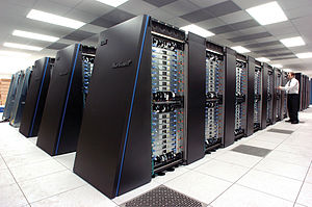
\includegraphics[width=390bp,height=220bp,keepaspectratio]{assets/visuals/lecture-1/slide-22-big-data-big-calculations-visual-01.png}}};

  \node[anchor=north,text width=830bp,align=center,inner sep=0pt] at (480,-468)
    {{\ArialFont\fontsize{9}{11}\selectfont\color{c7F7F7F}
      Original lecture visual montage. Current contexts: \href{https://ourworldindata.org/grapher/historical-cost-of-computer-memory-and-storage}{data storage} and the
      \href{https://mobook.github.io/MO-book/notebooks/04/08-traveling-salesman-problem.html}{MO-book TSP notebook}. Image creators and reuse rights remain to be verified.}};
  \ABWFooter{\insertframenumber}
\end{abwframe}
